%--------------------------------------------------------------------------------------------------
\subsection*{Motivation}
\begin{frame}[t]
    \frametitle{Motivation}
    \framesubtitle{Low Stakes}
    My go to exercise is running, \textbf{but...}\pause
    \begin{figure}
        \centering
        \begin{tikzpicture}[font={\scriptsize}]
            \node[align=center] (text_1) at (0,4) {I think my running shoes \\
                are getting \emph{worn}};
            \node (img_in) at (0, 1.25) {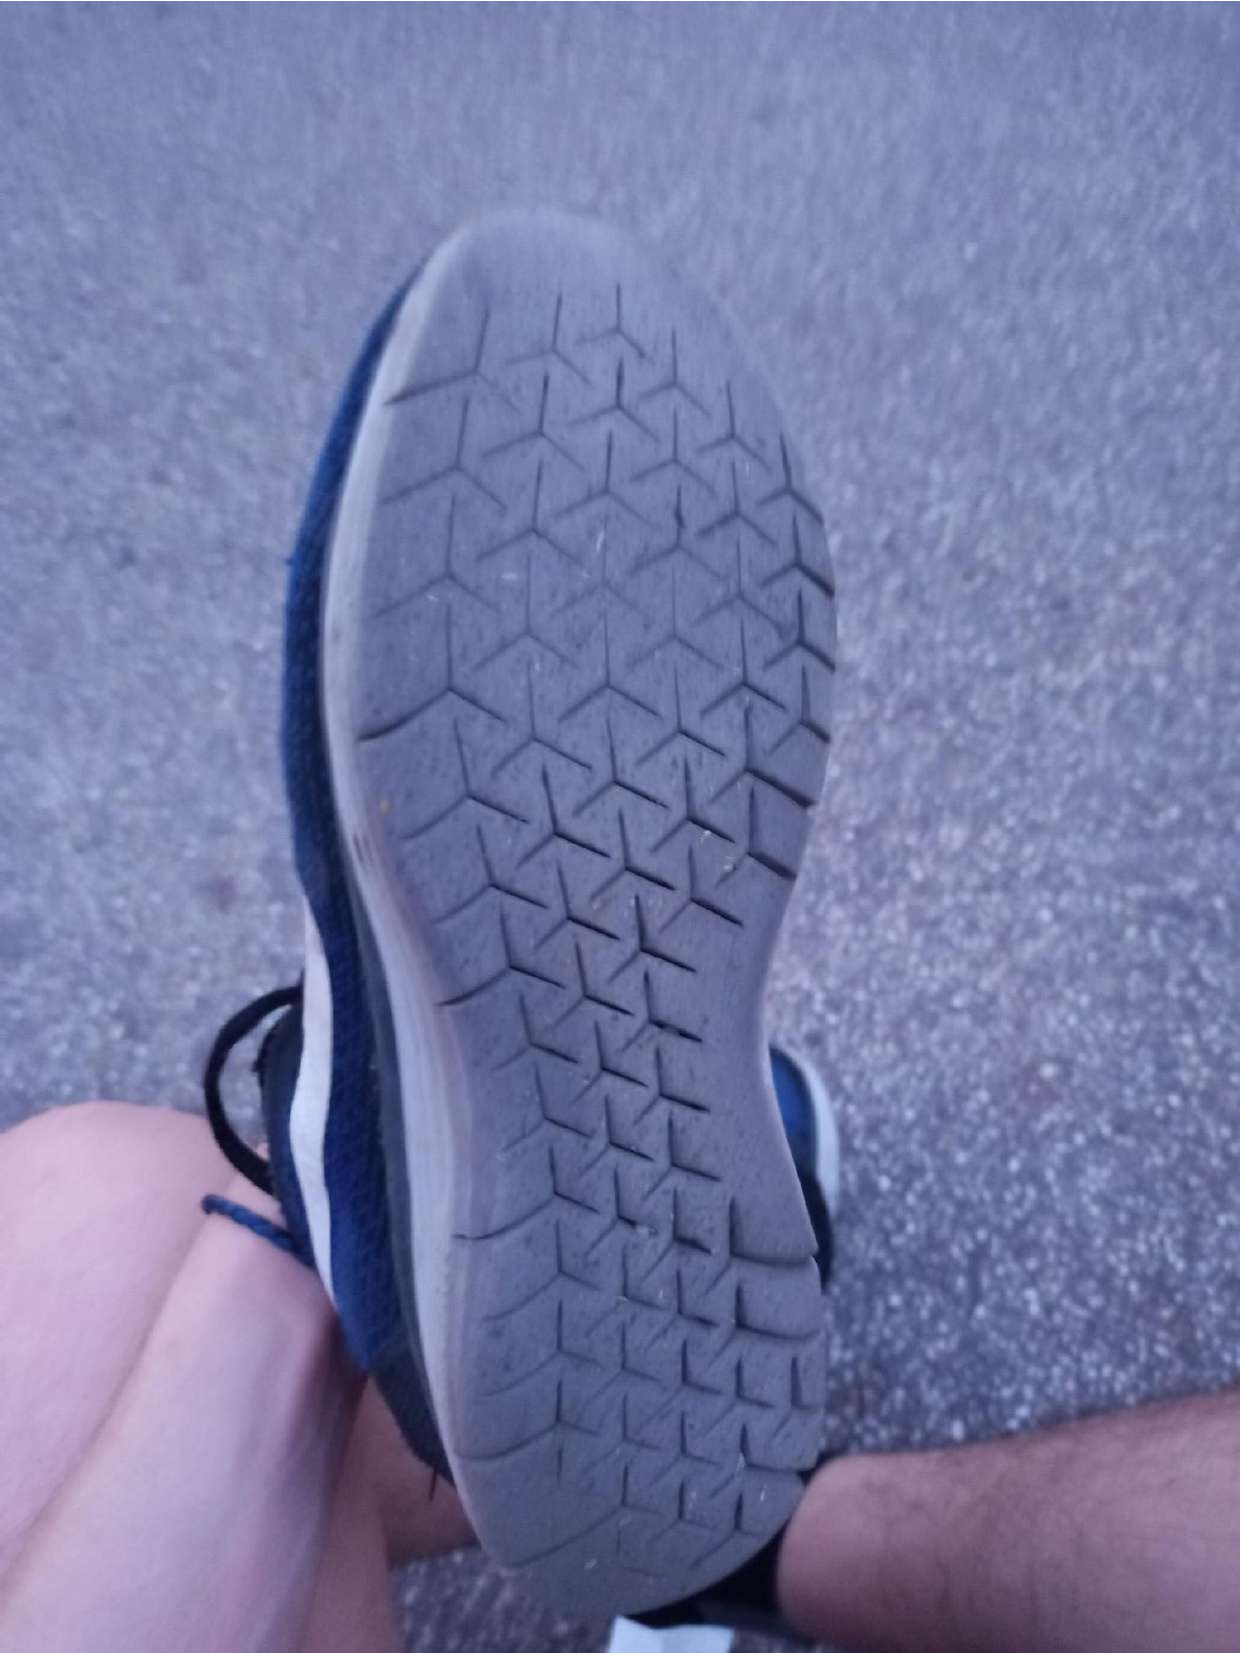
\includegraphics[scale=0.15]
                {fig/intro/motivation/lo_stakes/img/tired_boss.pdf}};
            \pause
            \node[align=center] (text_2) at (3.5, 4) {I want a replacement, \\ 
                 \emph{but} I know about\\machines, not shoes!};
            \node (img_shoe_raw) at (3.5,1.45) {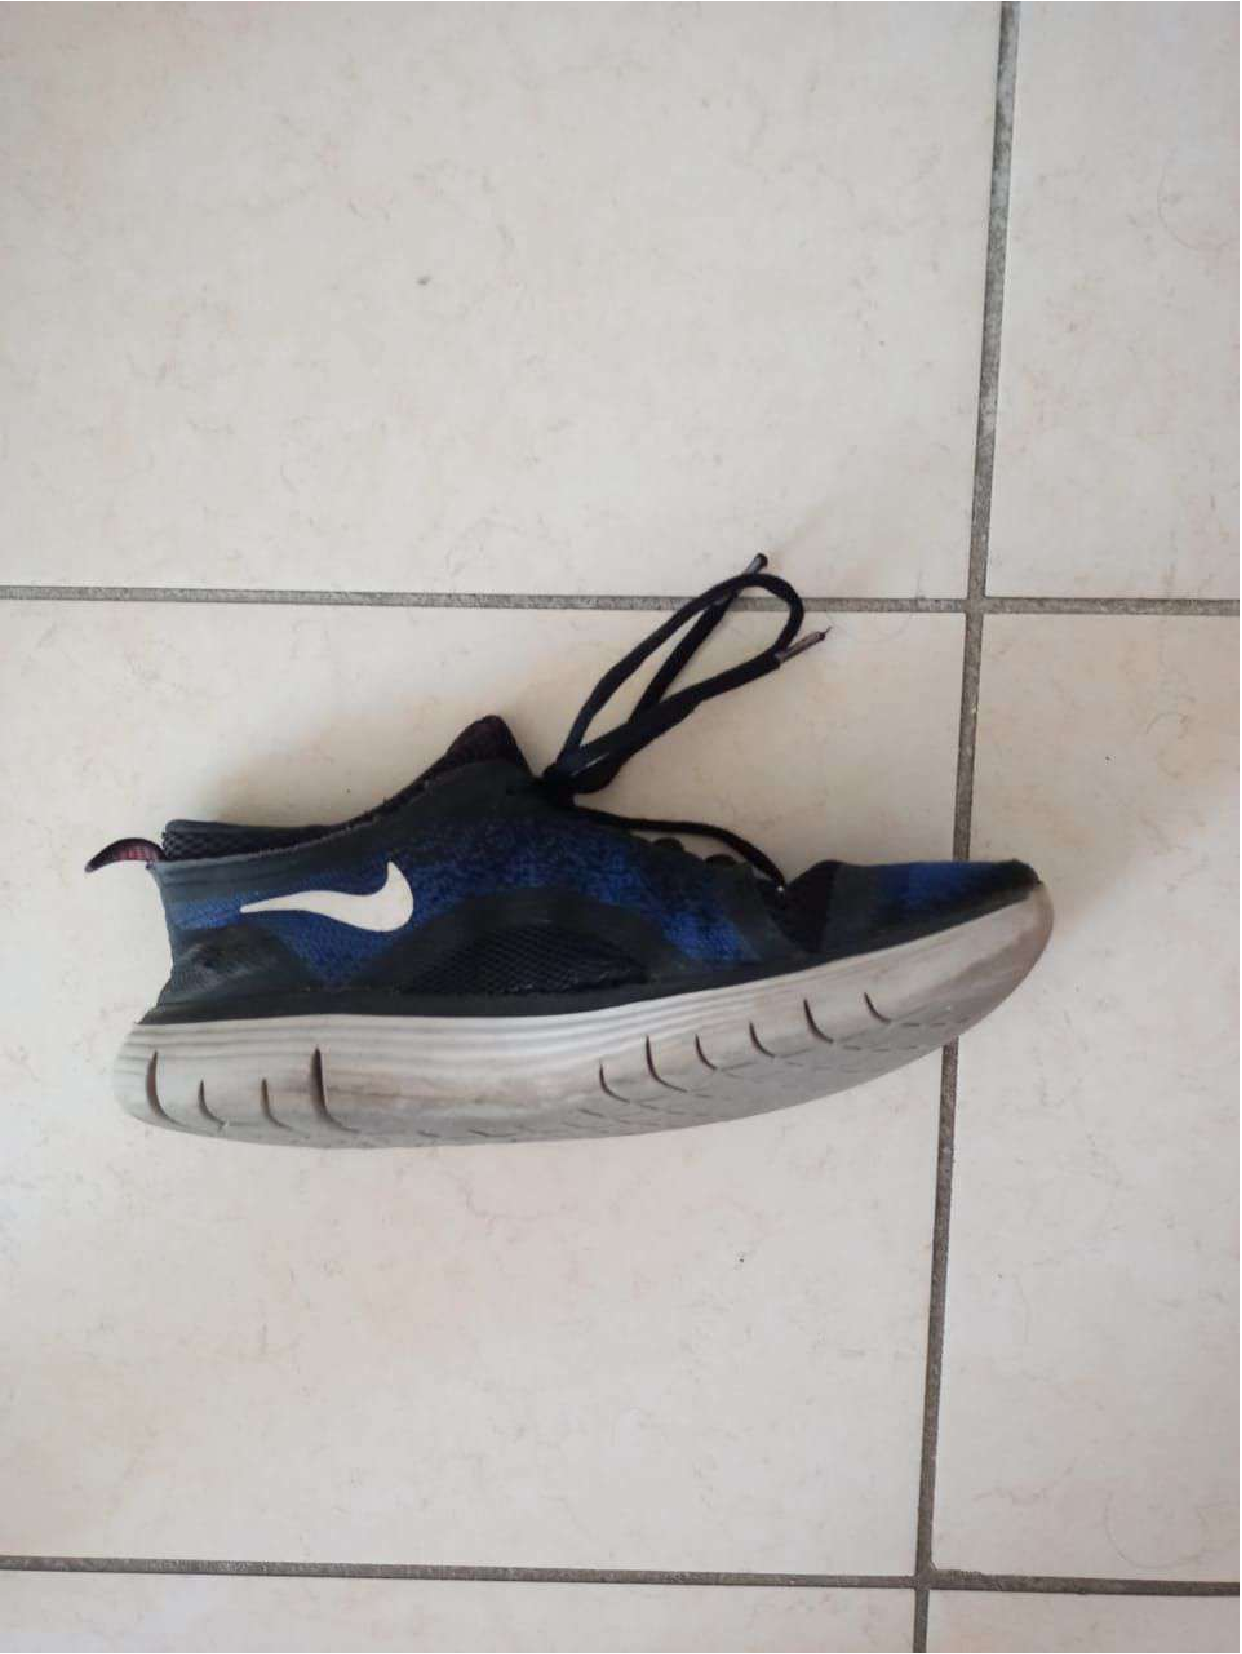
\includegraphics[scale=0.125]
                 {fig/intro/motivation/lo_stakes/img/shoe_current.pdf}};
            \pause
            \node[align=center] (text_5) at (3.5, -1) {My phone can \\
                \emph{identify} my current shoes};
            \node (img_zeros) at (3.5,1.45) 
                {
\includegraphics[scale=0.125]{fig/intro/motivation/lo_stakes/img/zeros_img.jpeg}};
            \node (img_idd) at (3.5,1.45) 
                {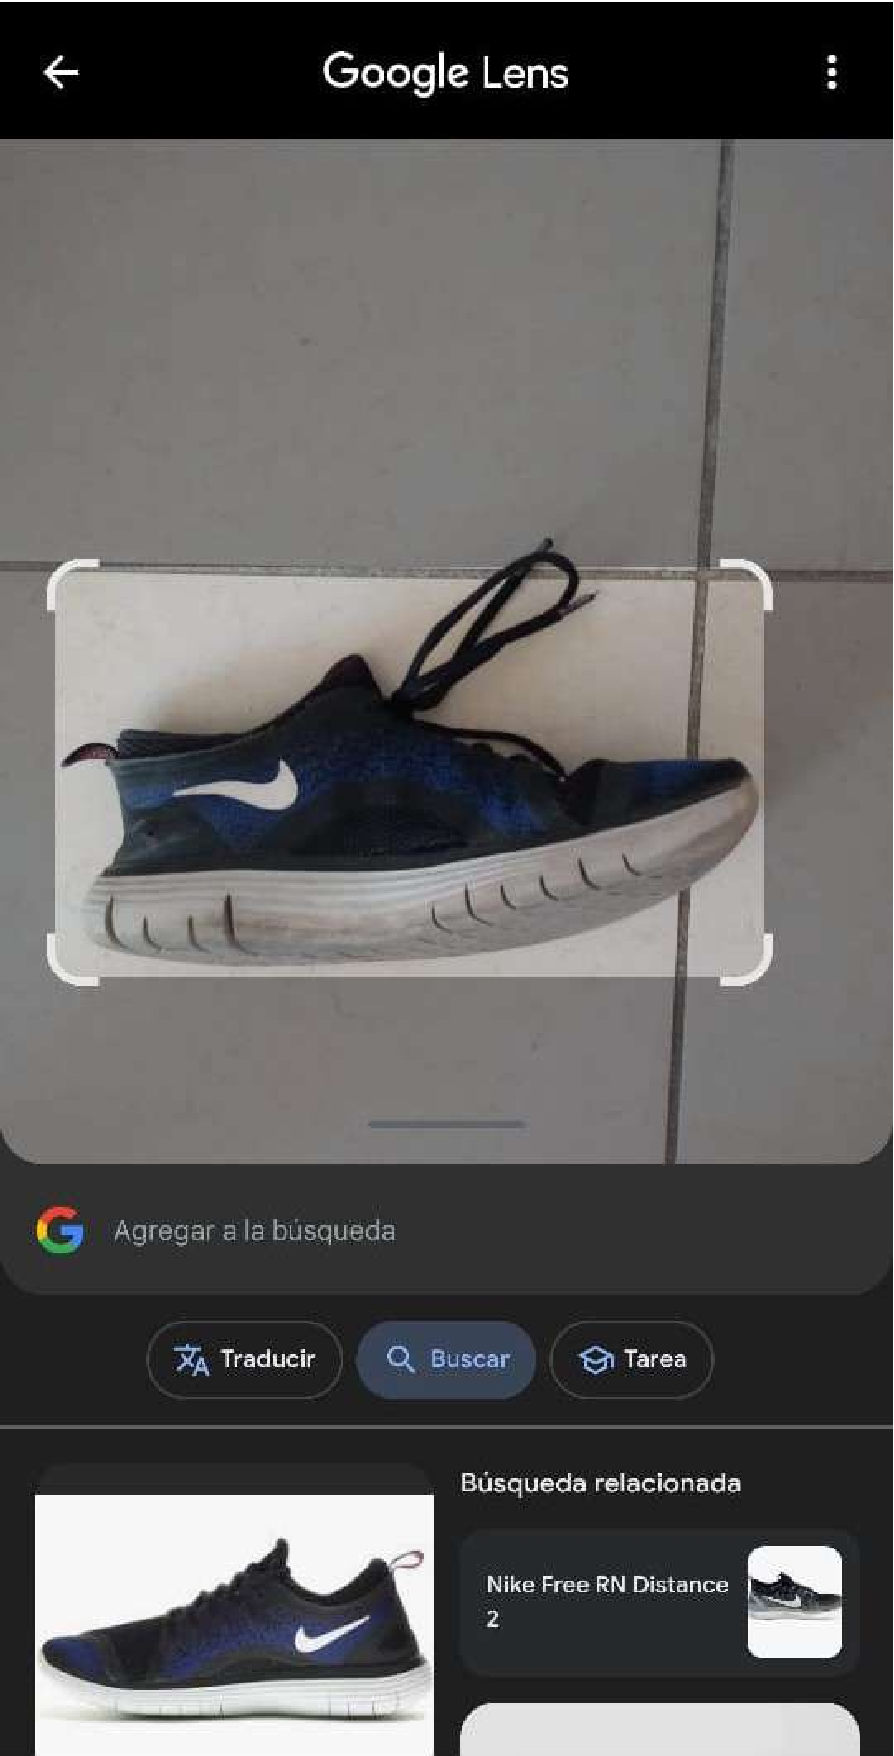
\includegraphics[scale=0.125]{fig/intro/motivation/lo_stakes/img/shoe_lens.pdf}};
            \pause
            \node[align=center] (text_brand_new) at (7, 3) {\emph{Nike Free RN Distance 2}};
            \node (img_brand_new) at (7, 1.75) 
                {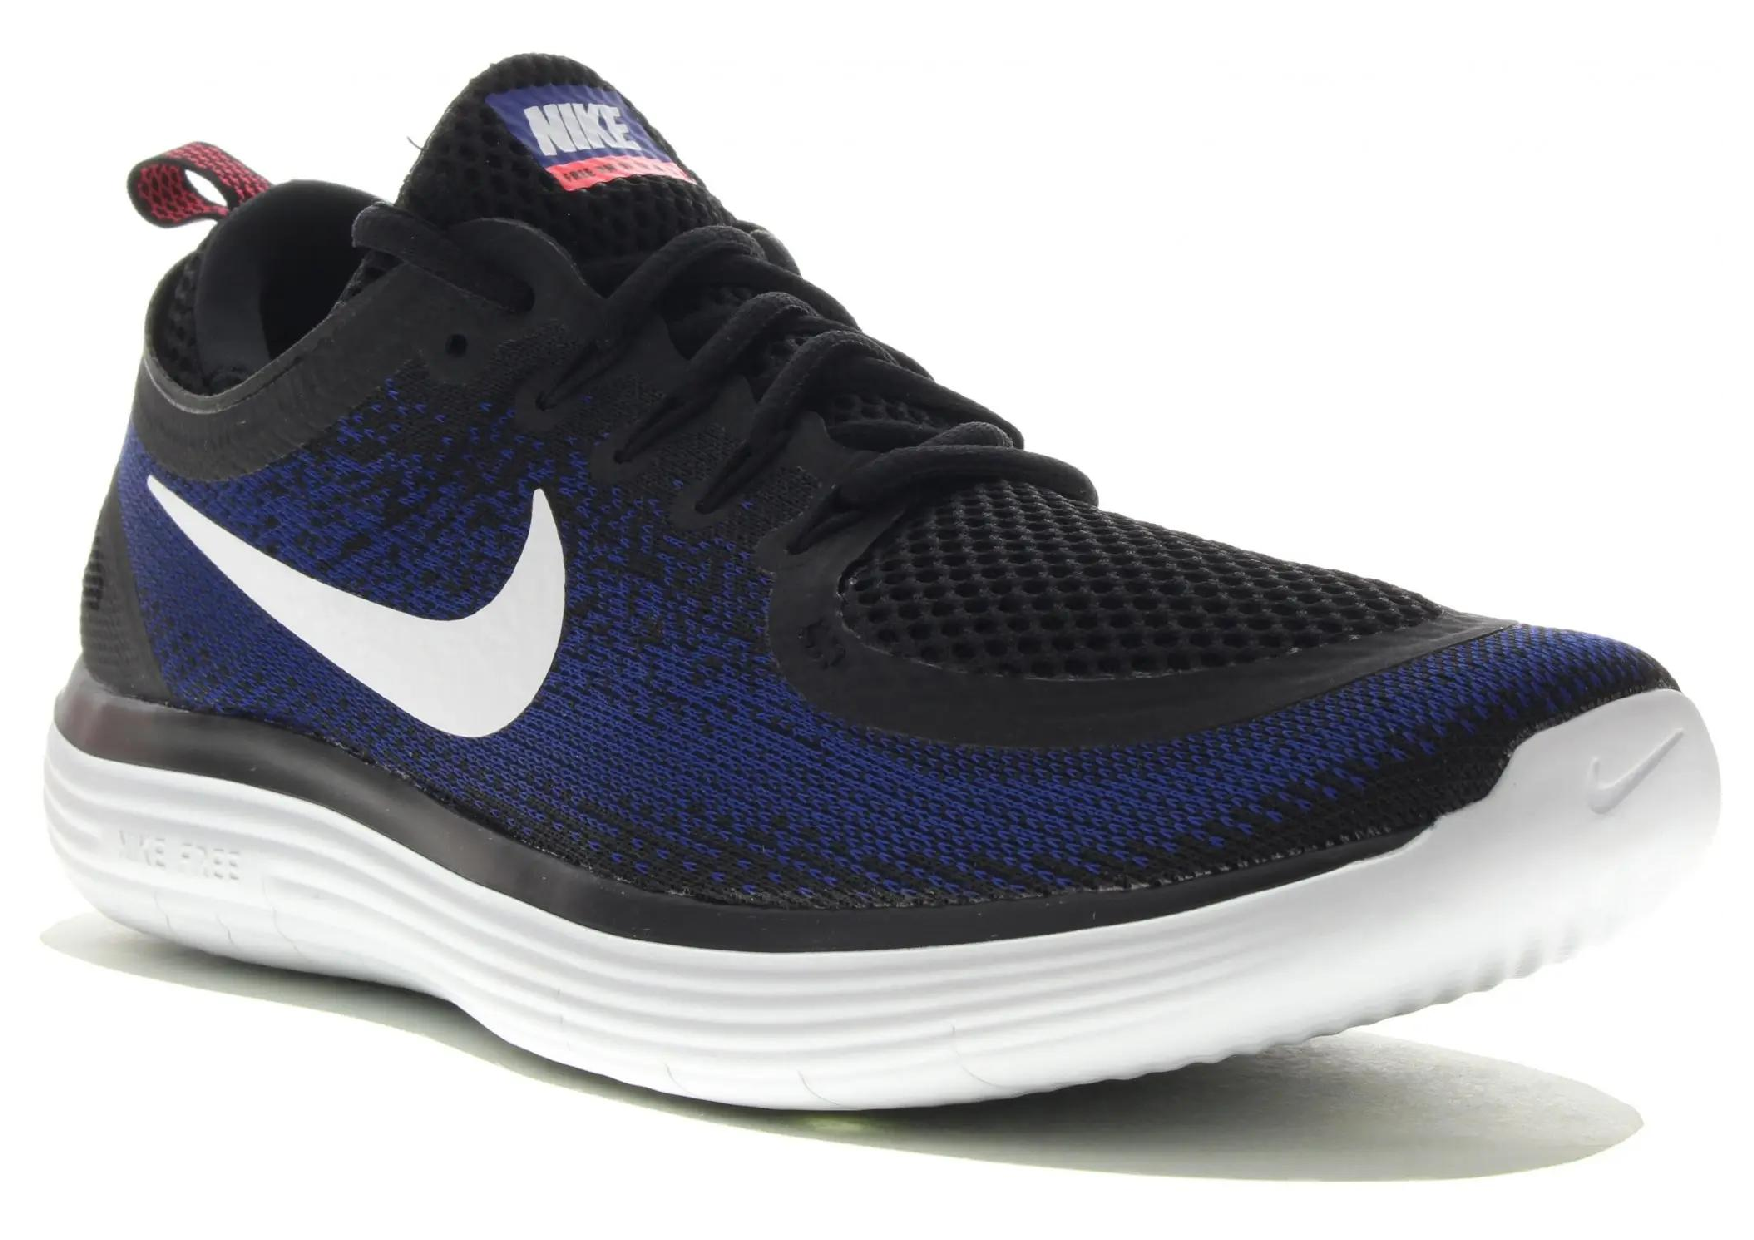
\includegraphics[scale=0.05]{fig/intro/motivation/lo_stakes/img/brand_new}};
            %\node[align=center] at (img_brand_new.south) {The \emph{Nike Free RN Distance 2}};
            \pause 
            \node (bigQ) at (7, 0) {\textbf{\emph{How} could my phone}\\
                \textbf{identify that model?}};
        \end{tikzpicture}        
    \end{figure}
\end{frame}
 %--------------------------------------------------------------------------------------------------
\begin{frame}[t]
    \frametitle{Motivation}
    \framesubtitle{Raising the stakes}
    Now let's consider riskier situations:
    \pause
    \begin{figure}
        \centering
        \begin{tikzpicture}[font={\scriptsize}]
            \node (cancer) at (current page.north west) 
                {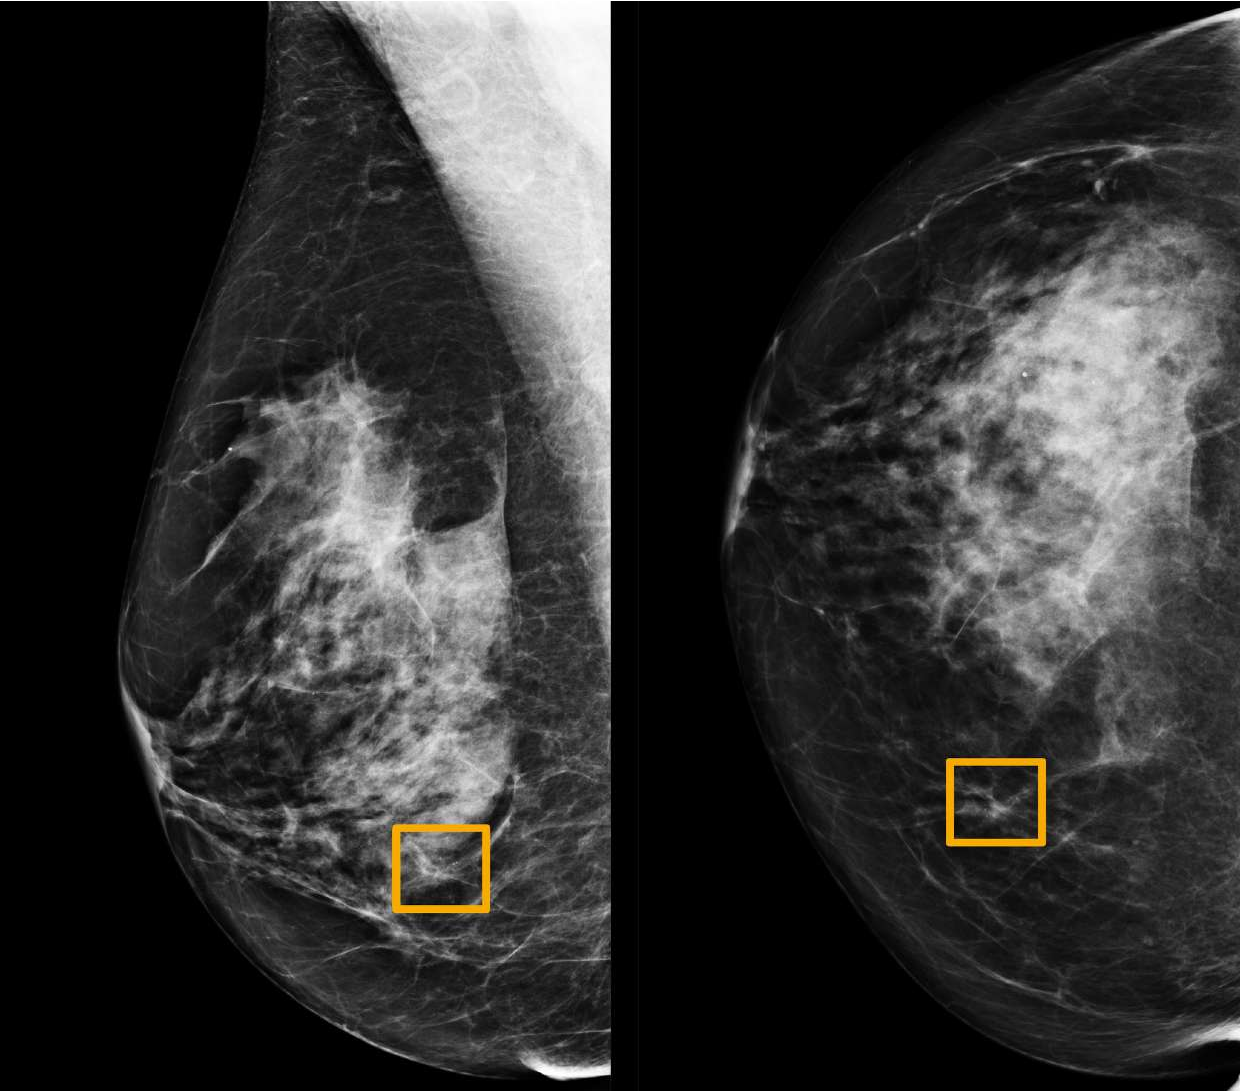
\includegraphics[scale=.2]{fig/intro/motivation/hi_stakes/img/breast_xray.pdf}};
            \pause
            \node (reid) at (cancer.south) {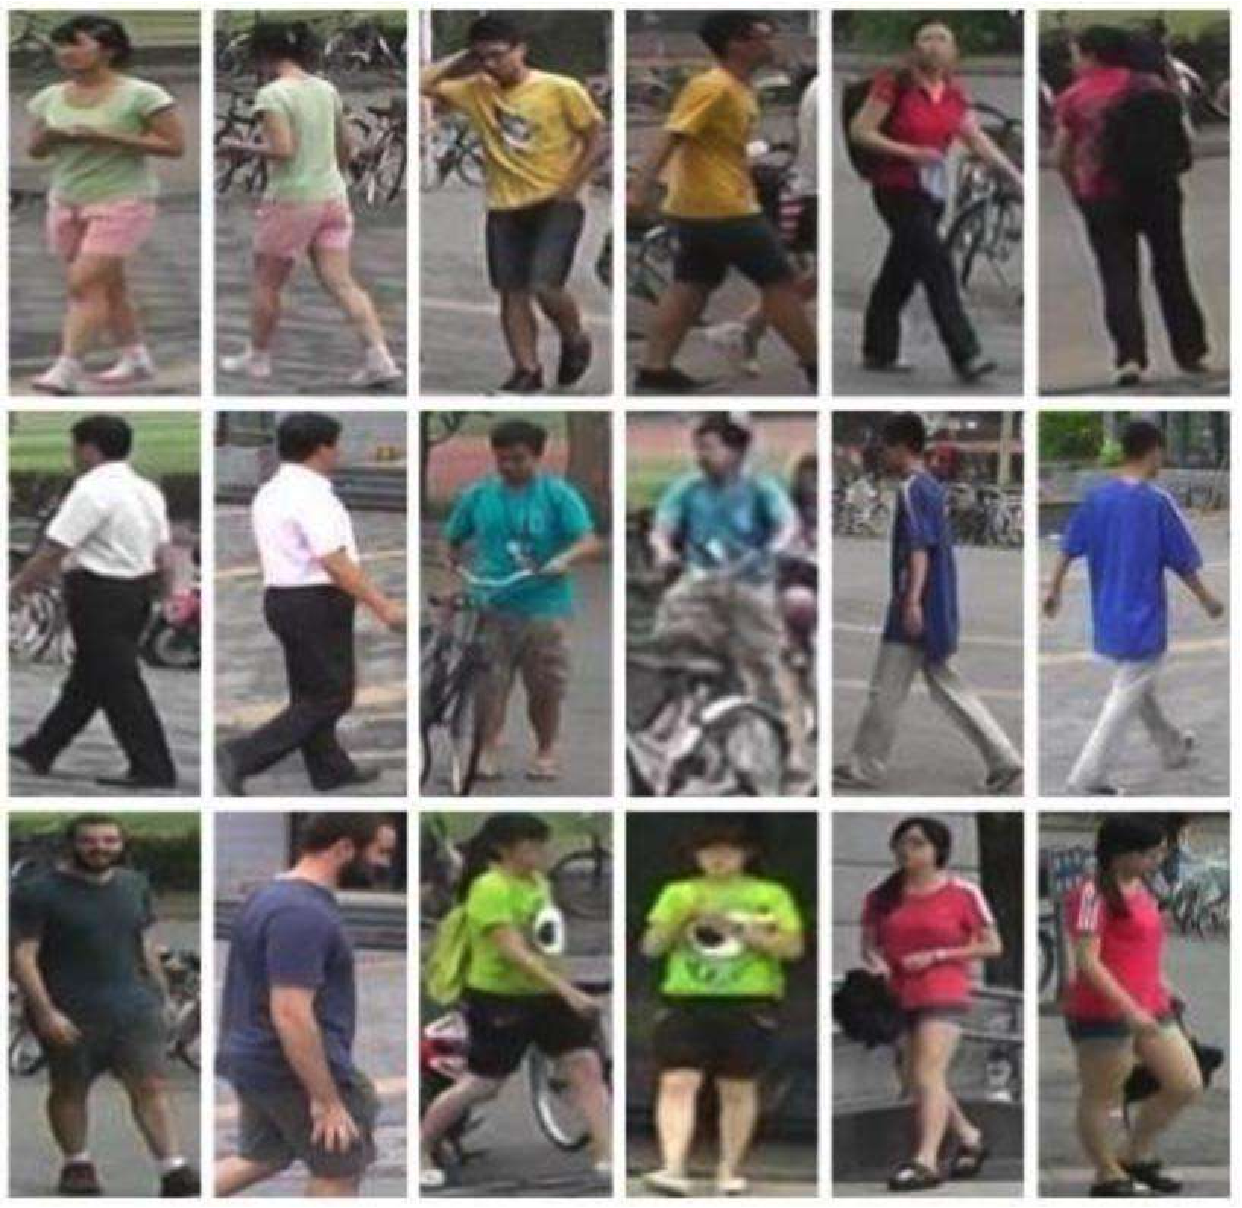
\includegraphics[scale=0.15]
                {fig/intro/motivation/hi_stakes/img/Market-1501.pdf}};
            \pause
            \node (roadkill) at (cancer.east) {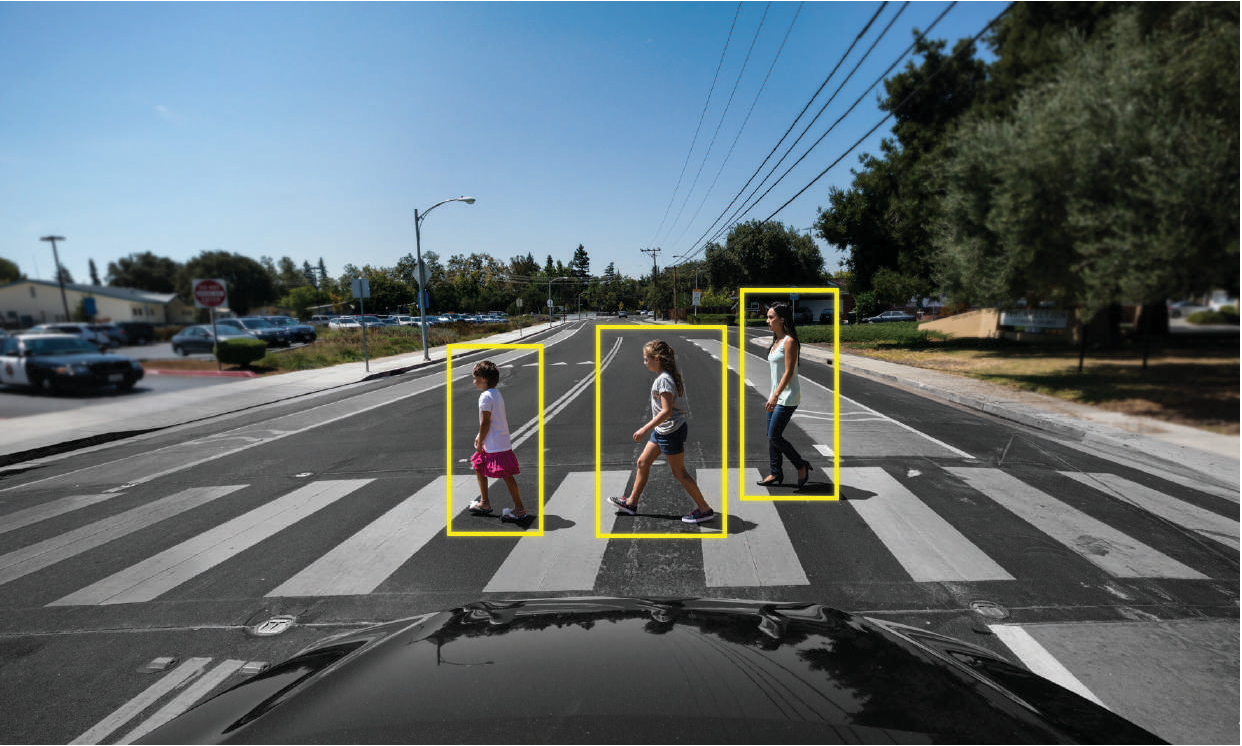
\includegraphics[scale=0.2]
                {fig/intro/motivation/hi_stakes/img/zebra_crossing.pdf}};
            
        \end{tikzpicture}
    \end{figure}
\end{frame}
 %--------------------------------------------------------------------------------------------------
 \begin{frame}[t]
    \frametitle{Motivation}
    \framesubtitle{Straight to the point}
    \begin{columns}[t]
        \column{0.5\textwidth}
        \begin{figure}
            \centering
            \begin{tikzpicture}[font={\scriptsize}]
                \node (cancer) at (current page.north west) 
                    {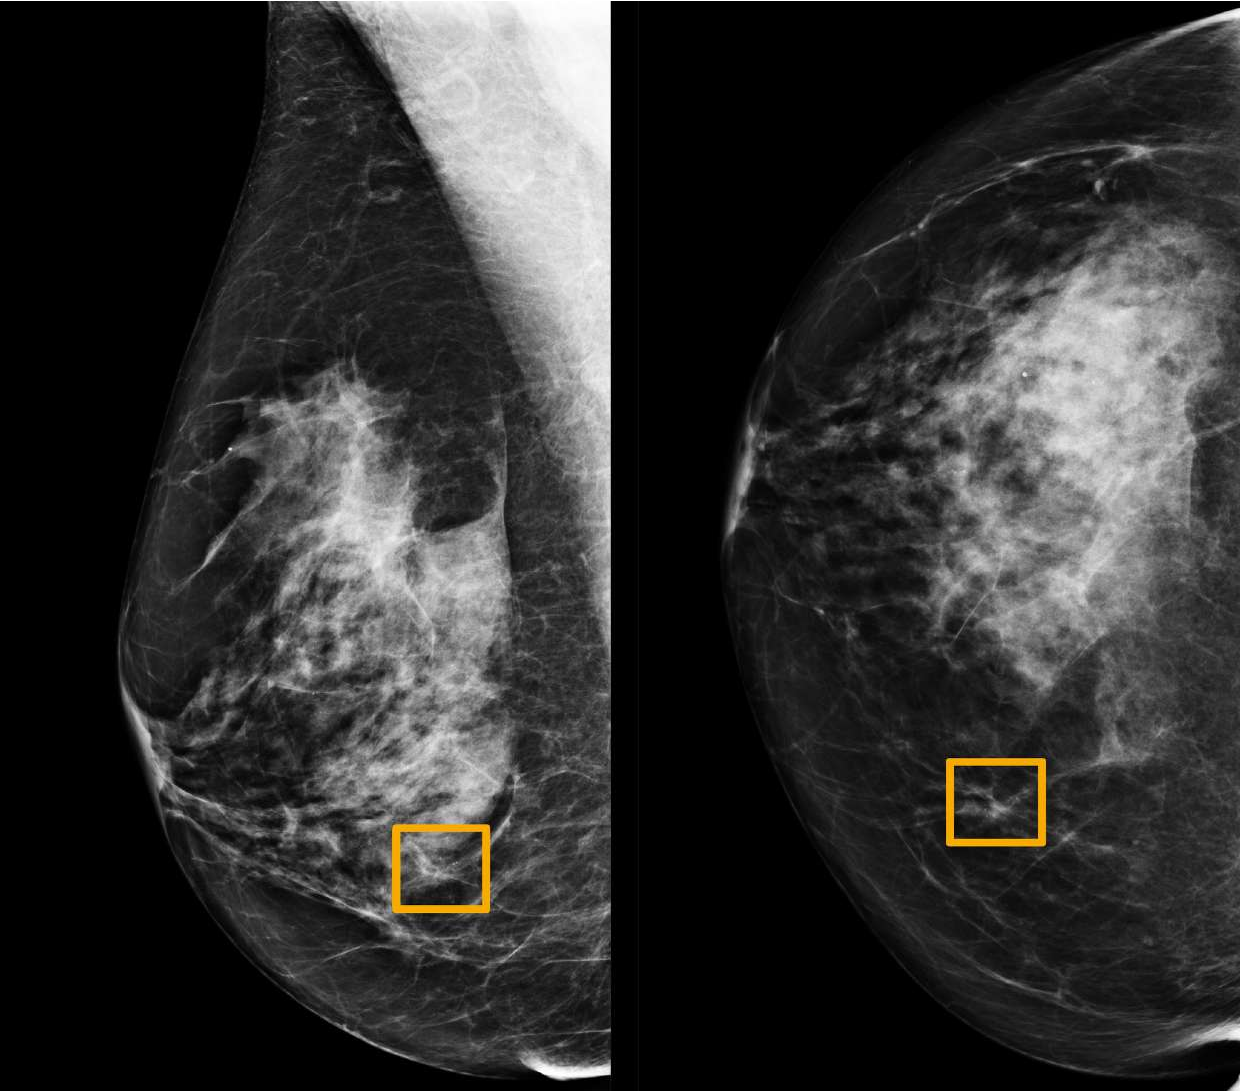
\includegraphics[scale=.2]{fig/intro/motivation/hi_stakes/img/breast_xray.pdf}};
                \node (roadkill) at (cancer.south) 
                    {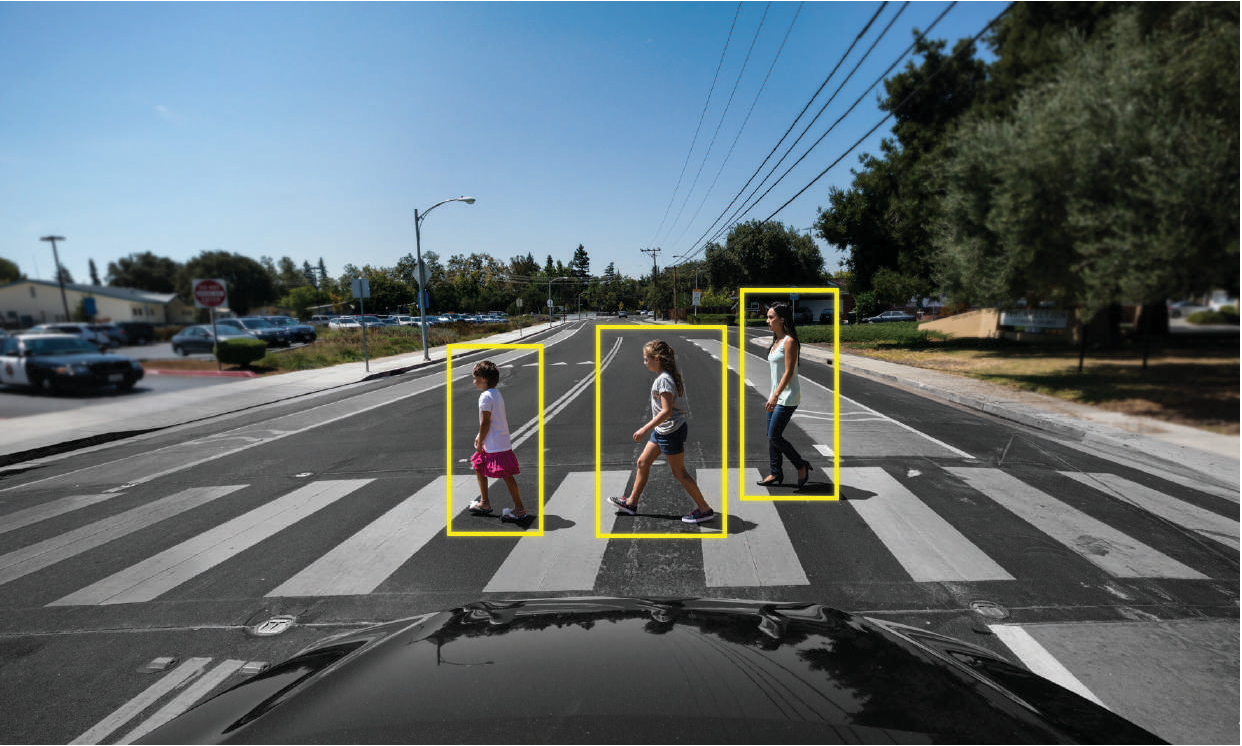
\includegraphics[scale=0.175]{fig/intro/motivation/hi_stakes/img/zebra_crossing.pdf}};
                \node (reid) at (roadkill.north east) 
                    {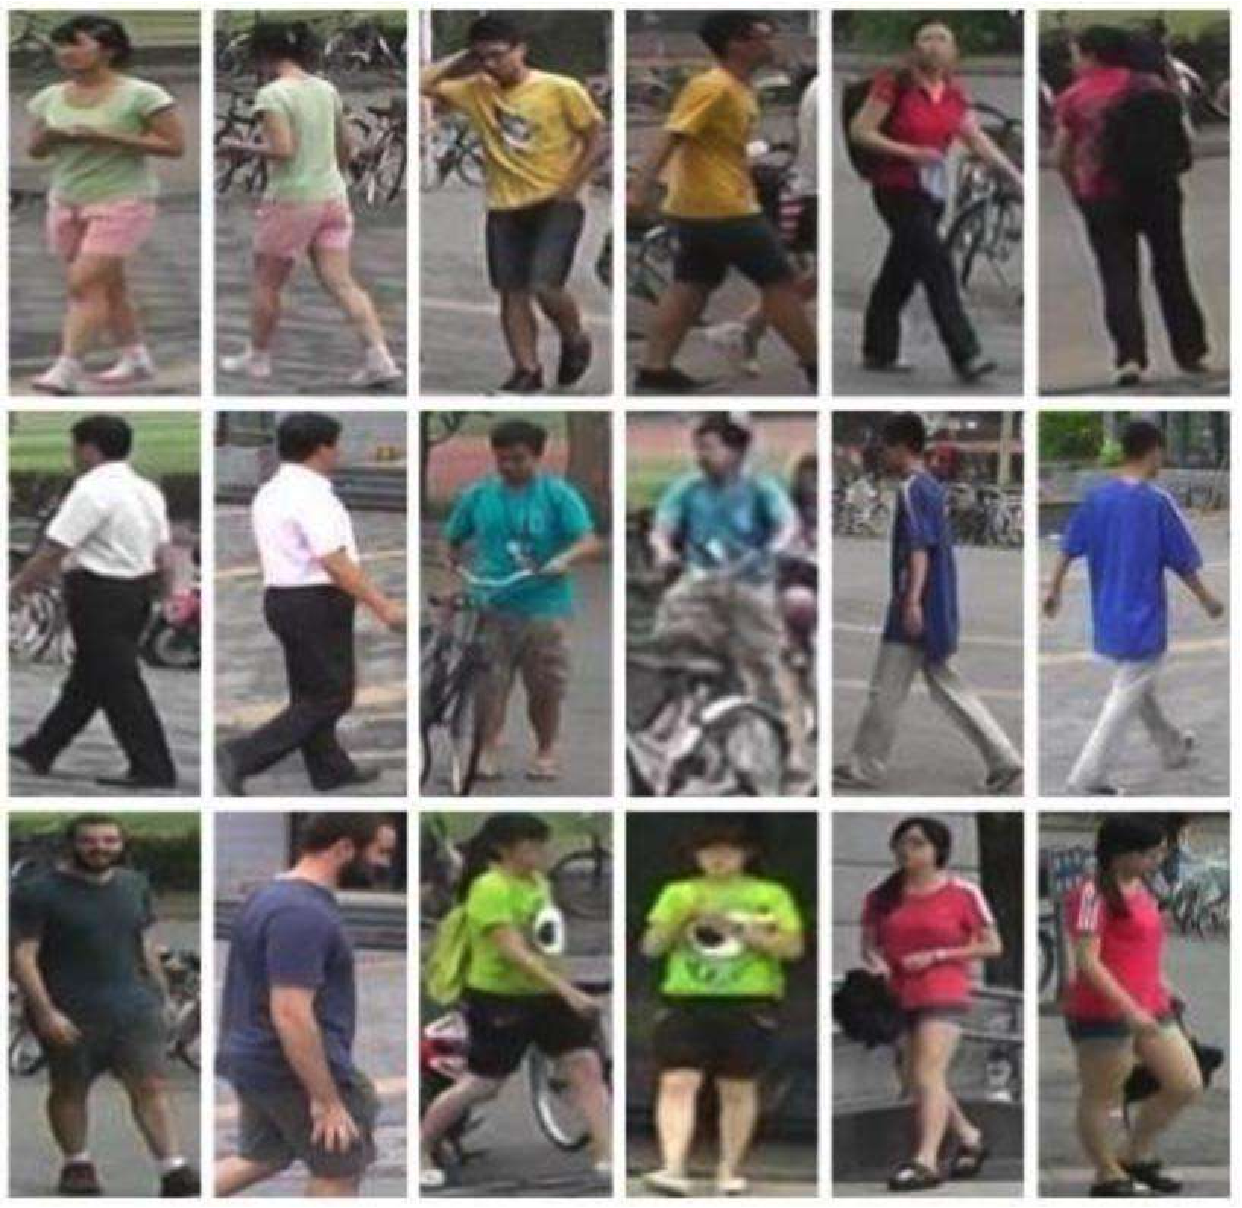
\includegraphics[scale=0.125]{fig/intro/motivation/hi_stakes/img/Market-1501.pdf}};                
            \end{tikzpicture}
        \end{figure}
        \column{0.5\textwidth}
            \begin{itemize}
                \item How do we \textbf{know how} a system works?\pause
                \item How do we \textbf{know how} safe a system is?\pause
                \item If a system fails, \textbf{who} is accountable?
            \end{itemize}
            We must \textbf{understand} the behaviour of these models.
        \end{columns}
 \end{frame}
 %--------------------------------------------------------------------------------------------------
\begin{frame}
    \frametitle{Step by step}
    \begin{columns}[c]
        \column{0.25\textwidth}
            \begin{center}
                Computation, Computer Vision and AI
            \end{center}
        \column{0.125\textwidth}
            \begin{center}
                $\rightarrow$
            \end{center}
        \column{0.25\textwidth}
            \begin{center}
                Explainable AI
            \end{center}
        \column{0.125\textwidth}
            \begin{center}
                $\rightarrow$                
            \end{center}
        \column{0.25\textwidth}
            \begin{center}
                Thesis objectives                
            \end{center}
    \end{columns}
\end{frame}
%--------------------------------------------------------------------------------------------------